En esta sección se presentan resultados obtenidos para la calibración usada, así como la obtención y análisis de los mapas de dosis que se obtuvieron.
\section{Calibración}
Como fue mencionado anteriormente, se irradiaron películas con dosis que se registran en la tabla \ref{tab:DosisIrra}, con su correspondiente incertidumbre, medidas con la cámara de ionización.\\

\begin{table}[]
	\centering
	\begin{tabular}{|l|l|l|}
		\hline
		UM& Dosis(Gy)    & Incertidumbre($10^{-5}$) \\ \hline
		21.6&0.201472 & 3.8\\ \hline
		54&0.504137 & 5.23 \\ \hline
		108&1.00825  & 35\\ \hline
		216&2.01783  & 22\\ \hline
		432&4.037486 & 31 \\ \hline
		648&6.0583   & 48\\ \hline
		864&8.08168  & 142\\ \hline
		1080&10.1056  & 140\\ \hline
		1296&12.132   & 10\\ \hline
		1620&15.168   & 10\\ \hline
		2160&20.229   & 10\\ \hline
	\end{tabular}
	\caption{Dosis irradiadas}
	\label{tab:DosisIrra}
\end{table}

Las películas resultantes después de la irradiación se muestran en la figura \ref{fig:peliculasIrradiacion}. Todas las películas fueron escaneadas en la misma sección del escáner para reducir efectos de posición en la transmitancia.\\
\begin{figure}[H]
	\centering
	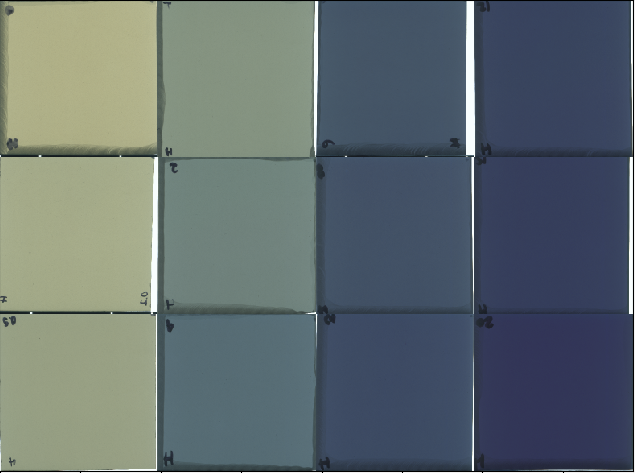
\includegraphics[width=0.7\linewidth]{images/peliculasIrradiadas.png}
	\caption{Películas EBT3 irradiadas con dosis entre 0 y 20 Gy. }
	\label{fig:peliculasIrradiacion}
\end{figure}

Para relacionar determinados niveles de transmitancias medidas en una película con la dosis que produjo la coloración, es necesario establecer una curva de calibración. En este caso, se correlacionaron los promedios de transmitancia en la misma región de interés de las tres películas irradiadas con la misma dosis con la dosis medida con la cámara de ionización aplicada en cada caso. Con estos valores, se establece la curva de calibración que se muestra en la figura \ref{fig:curvaFinal20} con sus respectivos parámetros.\\


\begin{figure}[H]
	\centering
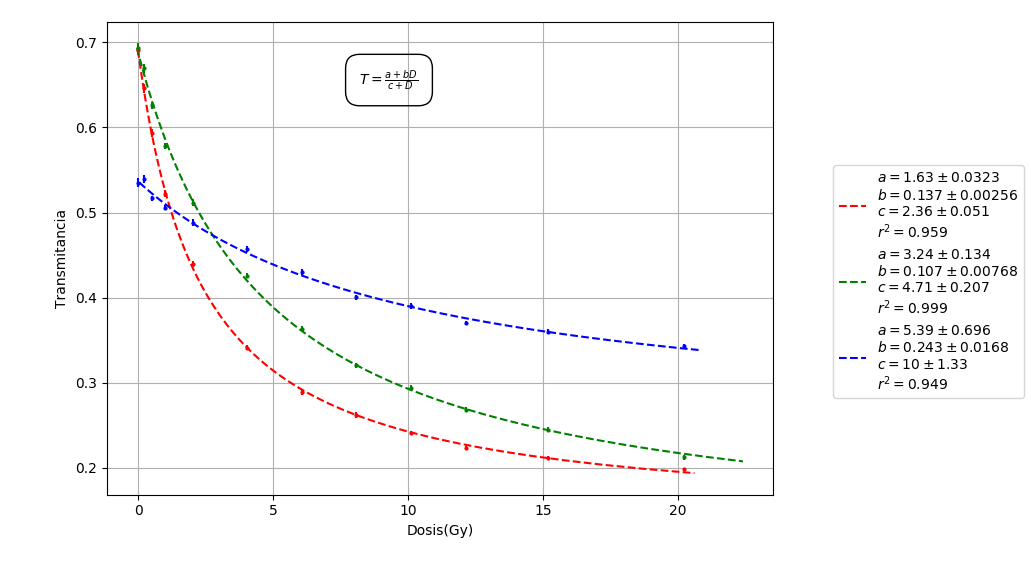
\includegraphics[width=\linewidth]{images/calibracionMulti0a20.png}
	
	\caption{Curva de calibración con dosis de 0 a 20 Gy. }
	\label{fig:curvaFinal20}
\end{figure}

En la cual se usó una curva del tipo 
\begin{equation}
D=\frac{AT+D}{T-C}.
\end{equation}\\

Según el manual del fabricante, las películas EBT3 son aptas para un rango inferior a 30 Gy, sin embargo su comportamiento en los canales rojo y verde es ligeramente diferente en el rango de 10 a 30 Gy, por lo que se prefieren omitir los últimos tres puntos de dosis, puesto que la película está entrando en la región de saturación en esta región. Esto se realiza para obtener un mejor ajuste con la curva propuesta, ya que en esta región de dosis la curva propuesta describe mejor el comportamiento de la película.  Además, estos puntos no aportan información adicional a los propósitos del trabajo, puesto que los planes que serán examinados no conllevan dosis tan altas. De esta manera se obtiene la curva que se muestra en la figura \ref{fig:curvaFinal}\\

\begin{figure}[H]
	\centering
	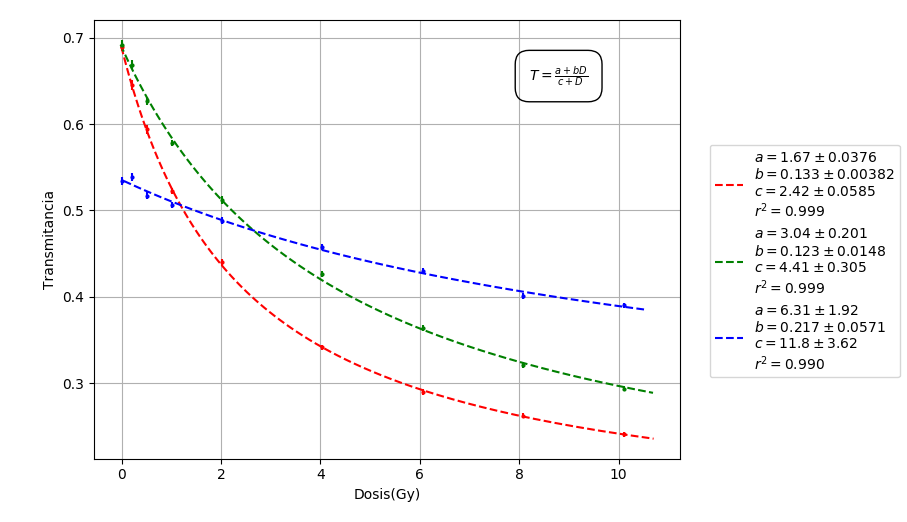
\includegraphics[width=\linewidth]{images/calibracionMulti.png}
	\caption{Curva de calibración con dosis de 0 a 10 Gy. }
	\label{fig:curvaFinal}
\end{figure}

En esta, se evidencia que las curvas ajustadas describen mejor los datos, puesto que no se ha alcanzado la región de saturación, lo cual se demuestra con los mejores test de ajuste $\chi ^2$ calculados. También se evidencia que el canal que menos se ajusta y tiene un comportamiento más por fuera de lo esperado es el azul, consecuente con el hecho que en esta longitud de onda los cambios de coloración de la película son menores. Estas curvas son las que se usan a lo largo del trabajo para calcular mapas de dosis.\\

También se probaron más curvas sugeridas en la literatura, sin embargo, la que mejor se ajustó a los datos con las películas EBT3, en este rango de dosis, fue la anteriormente mencionada. En la figura \ref{fig:CurvasAdicionales} se muestran otros dos ajustes con las respectivas formas de la función de ajuste y su bondad de ajuste.


\begin{figure}[H]
	\centering
	\subfloat[Curva cubica]{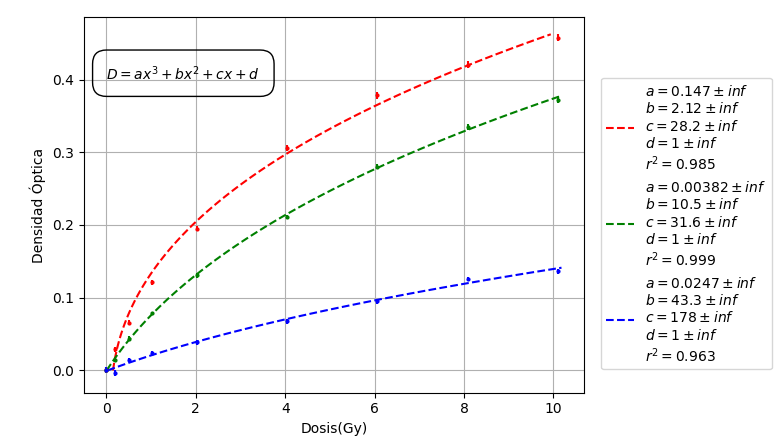
\includegraphics[width=0.7\textwidth]{images/calibracionCubica.png}\label{fig:cubic}}
	\hfill
	\subfloat[Curva exponencial]{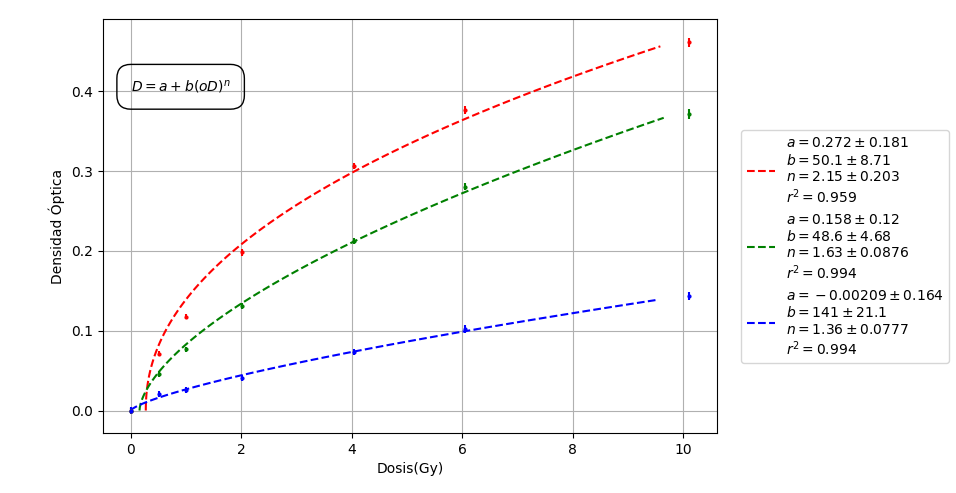
\includegraphics[width=0.7\textwidth]{images/curvaCalibracionMalaExponencial.png}\label{fig:expo}}
	\caption{Curvas de calibración con otro tipo de funciones}
	\label{fig:CurvasAdicionales}
\end{figure}

Acá, en la curva \ref{fig:cubic} se ajustó a una función cúbica. Similarmente, en la curva \ref{fig:expo} se realizó un ajuste a una función exponencial que resultó de menor calidad, comparado con la función racional usada inicialmente. Se debe notar que, en este caso, las curvas relacionan las cantidades  de densidad óptica con dosis absorbida y no de transmitancia directamente.\\

Finalmente, la única curva para realizar el  procedimiento de calibración multicanal fue la curva propuesta inicialmente, esto dado que las demás son susceptibles a errores numéricos que causan inestabilidad en el método de minimización usado. Estos errores numéricos son causados por la respuesta descontrolada de la función a pequeños cambios en sus parámetros, lo que hace que los métodos numéricos usados no converjan con facilidad.


\section{Efectos de diversos parámetros}

Para evaluar los efectos de diversos factores en la digitalización y posterior conversión de películas radicrómicas en mapas de dosis, se estudiaron varios ejemplos. \\

En primer lugar, se estudió el efecto de la posición en el área de escaneo en la transmitancia medida con el escáner. Para esto se examina el comportamiento de la transmitancia de una película sin irradiar a lo largo de un perfil horizontal y vertical en esta. Con este objetivo, la digitalización de la placa que se muestra en la figura \ref{fig:fondoCero} se transformó en un mapa de dosis, al cual se le extrajeron los perfiles horizontales y verticales que se muestran en la figura \ref{fig:perfiles}.\\

\begin{figure}[H]
	\centering
	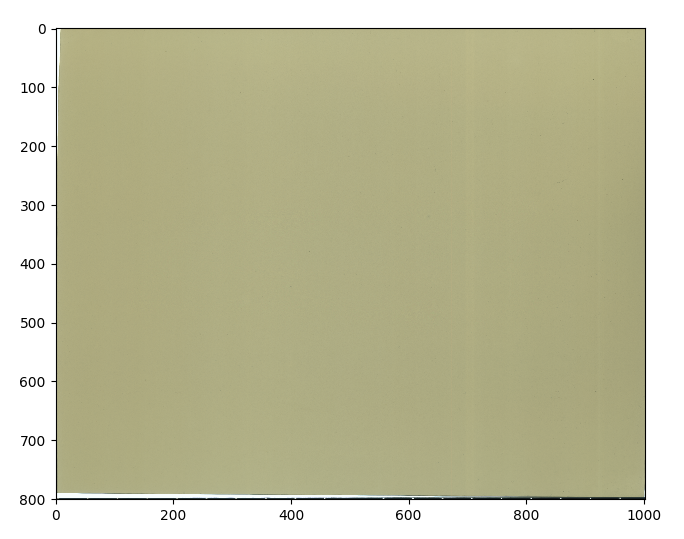
\includegraphics[width=0.7\linewidth]{images/imagenFondoCero.png}
	\caption{Película EBT3 sin irradiar. }
	\label{fig:fondoCero}
\end{figure}

\begin{figure}[H]
	\centering
	\subfloat[Perfil horizontal.]{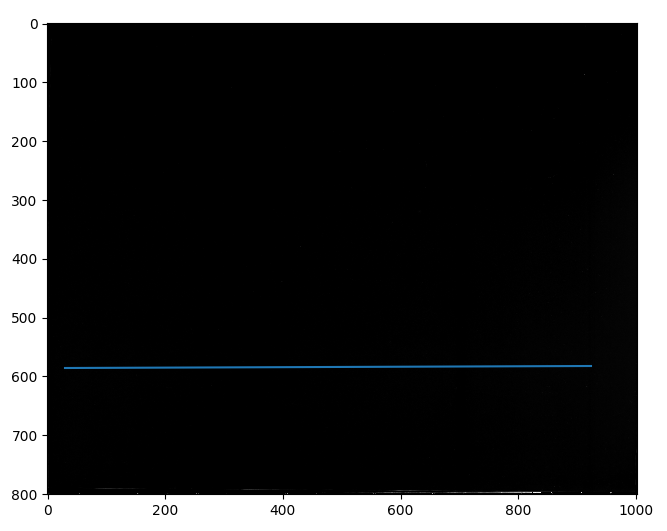
\includegraphics[width=.45\linewidth]{images/imagenPerfilMapaCeroHorizontal.png} }\qquad

	\subfloat[Perfil vertical.]{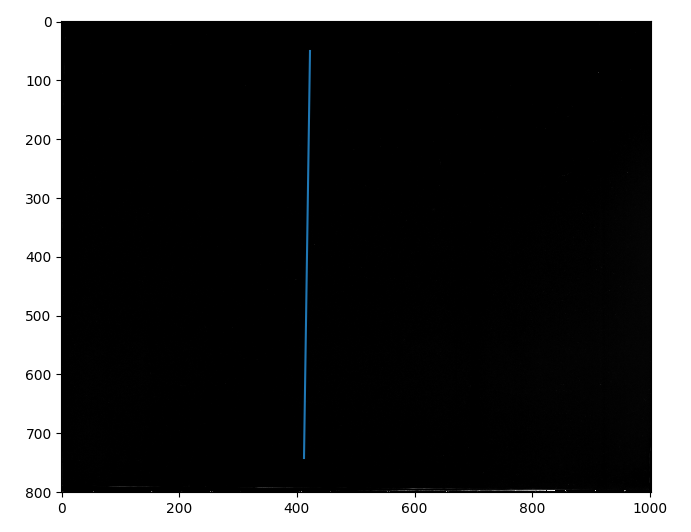
\includegraphics[width=0.45\linewidth]{images/imagenPerfilMapaCeroVertical.png}}\\

		\subfloat[Perfil horizontal de dosis.]{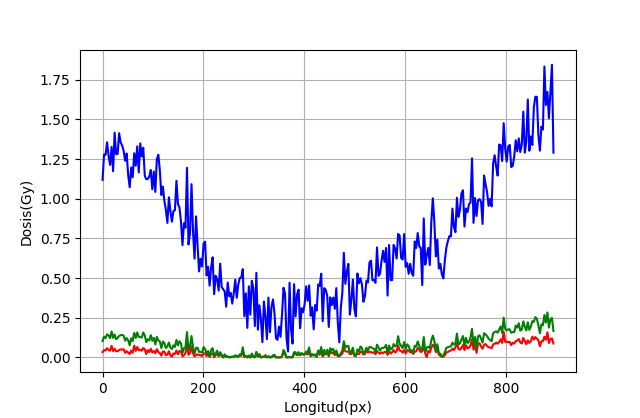
\includegraphics[width=0.45\linewidth]{images/perfilDosisCeroHorizontal.png}}\qquad
\subfloat[Perfil vertical de dosis.]{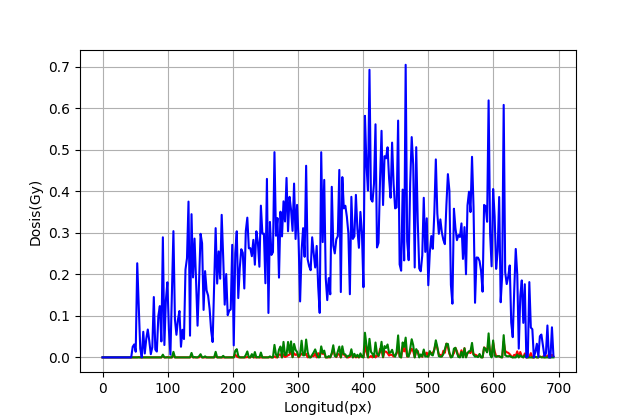
\includegraphics[width=0.45\linewidth]{images/perfilDosisCeroVerticalEnCentro.png}}
	\caption{Perfiles de dosis de película sin irradiar.}
	\label{fig:perfiles}
\end{figure}



En estos perfiles se evidencia un sesgo sistemático en la dosis predicha para la película en cada punto. Se esperaría que, salvo variaciones muy pequeñas, los perfiles de dosis siempre dieran valores cercanos a cero. Sin embargo, se observan varios comportamientos defectuosos reportados en la literatura. Se evidencia que en los tres canales de color se sobre-estima la dosis cuando el punto de estimación está lejos del eje central del escáner, es decir, cerca de los bordes.\\

También, se evidencia que el canal azul proporciona medidas erradas de dosis por la poca sensibilidad que tiene la película en ese rango de dosis, lo que permite decir que no debe ser usado para otros objetivos más que la calibración multicanal.\\

Otra propiedad que permite evidenciar estos perfiles, es la gran cantidad de ruido que mide el escáner, lo cual se ve en las grandes variaciones locales en los perfiles de dosis. Esto es consecuencia de varios factores, el principal de ellos son los pixeles defectuosos que el escáner pueda tener. Para identificar estos pixeles defectuosos, se cubrió el área de escaneo que se estaba usando con abundante cartulina negra, obteniendo la imagen escaneada que se muestra en la figura \ref{fig:fondoNegro}. En detalle se observan los pixeles absorben luz cuando no deberían. \\

\begin{figure}[H]
	\centering
	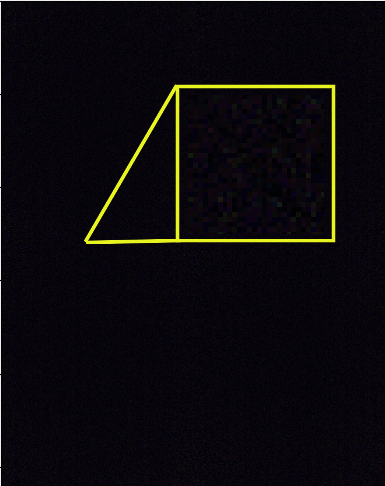
\includegraphics[width=0.7\linewidth]{images/fonRuido.png}
	\caption{Pixeles defectuosos del escáner }
	\label{fig:fondoNegro}
\end{figure}

Para corregir parte de este ruido, en las posteriores tomas se escaneó cada imagen múltiples veces, lo que reduce la cantidad de pixeles defectuosos.\\

Para continuar realizando pruebas en los métodos usados, se analiza el cuadrado de 5 Gy de 10x10 cm que se irradió. La película resultante se muestra en la figura \ref{fig:cuadrado5Gy}. En este se muestran los puntos fiduciales que se usan para identificar el eje del campo.\\

\begin{figure}[H]
	\centering
	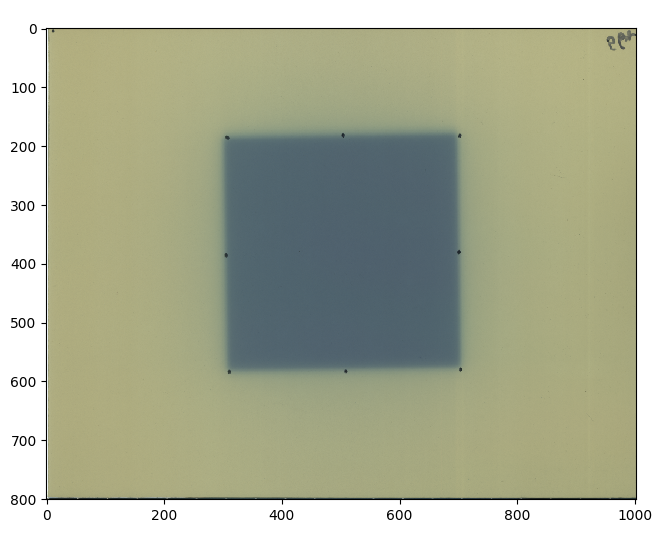
\includegraphics[width=0.7\linewidth]{images/peliculaCuadrado.png}
	\caption{Película irradiada con cuadrado de 5 Gy }
	\label{fig:cuadrado5Gy}
\end{figure}

Este cuadrado sirve para identificar fácilmente las ventajas del método multicanal con respecto a la calibración mediante canales individuales. En la figura \ref{fig:MapaCuadrado} se muestra el mapa de dosis del cuadrado obtenido junto con la separación que este método realiza de las partes de la transmitancia que son independientes de la dosis que se absorbió.\\
\begin{figure}[H]
	\centering
	\subfloat[Mapa de dosis del cuadrado de 5 Gy]{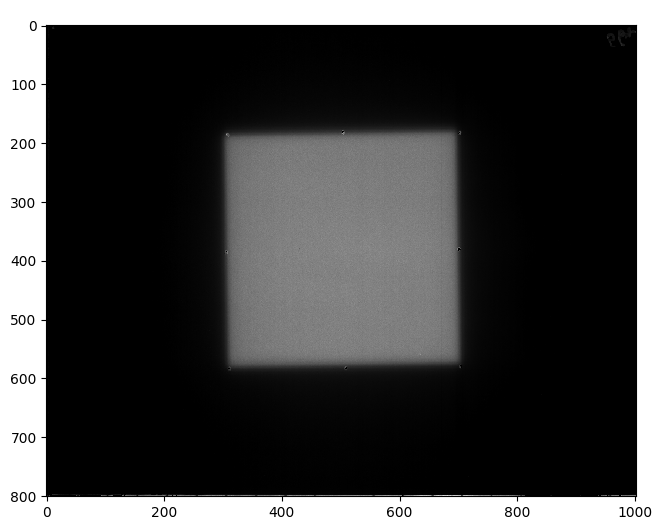
\includegraphics[width=0.5\textwidth]{images/mapaCuadradoConMulticanal.png}\label{fig:MapaCuadradoMulti}}
	\hfill
	\subfloat[Defectos de la película obtenidos con el método multicanal]{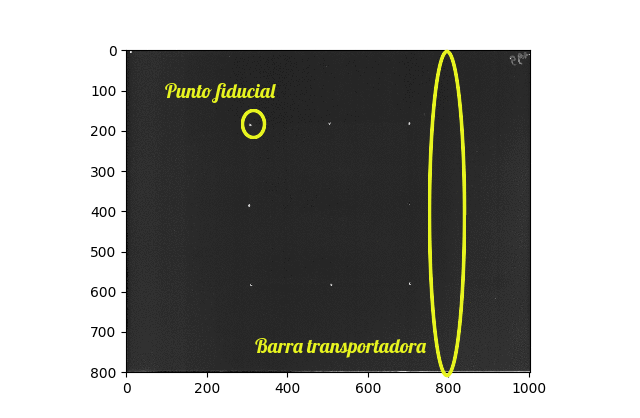
\includegraphics[width=0.8\textwidth]{images/fondoCuadradoConLabel.png}\label{fig:fondoCuadrado5Gy}}
	\caption{Mapa de dosis obtenido con el método multicanal}
	\label{fig:MapaCuadrado}
\end{figure}

En el mapa de defectos, se encuentran tanto los puntos fiduciales, como las barras transportadoras propias del escáner. Estas componentes ya no son tenidas en cuenta en el cálculo de dosis de cada punto. Esto resulta finalmente en un mapa de dosis más limpio, libre de una gran parte de irregularidades y efectos asociados a inhomogeneidades de la película.\\

Es posible comparar los perfiles de dosis sobre una línea que pasa por el centro de los cuadrados obtenidos con canales individuales y usando el método multicanal. En la figura \ref{fig:perfilesMapaCuadrado} se muestran perfiles centrales obtenidos con cada método. Se observa cómo se reduce el ruido con el método multicanal, resultando en una medida fiable de la dosis obtenida en cada punto. 
\begin{figure}[H]
	\centering
	\subfloat[Perfil de dosis central con método de un solo canal]{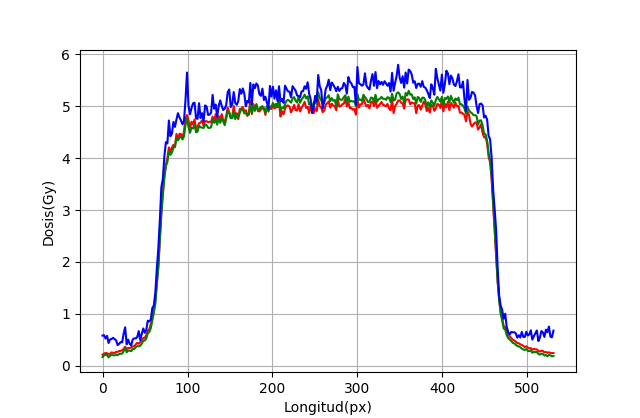
\includegraphics[width=0.7\textwidth]{images/perfilDosisCuadradoUnoSolo.png}\label{fig:perfilSolo}}
	\hfill
	\subfloat[Perfil de dosis central con método multicanal ]{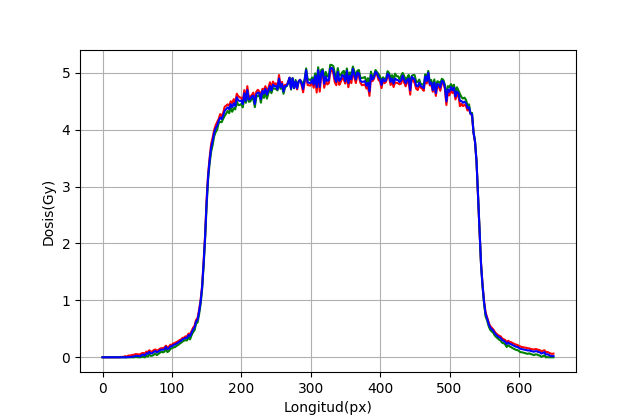
\includegraphics[width=0.7\textwidth]{images/perfilDosisCuadradoMulticanal.png}\label{fig:perfilMultiple}}
	\caption{Perfil central de dosis en película con cuadrado de 5 Gy}
	\label{fig:perfilesMapaCuadrado}
\end{figure}

Otra manera de observar la superioridad del método multicanal sobre el método de un solo canal es observar el mismo perfil, que se muestra en la figura \ref{fig:perfilSolo}, sobre la película sin irradiar como en la figura \ref{fig:perfilCero} pero ahora en el mapa calculado con la calibración multicanal. Aquí, se evidencia también que este método es útil para corregir la sobreestimación debida a la cercanía al borde del escáner.\\

\begin{figure}[H]
	\centering
	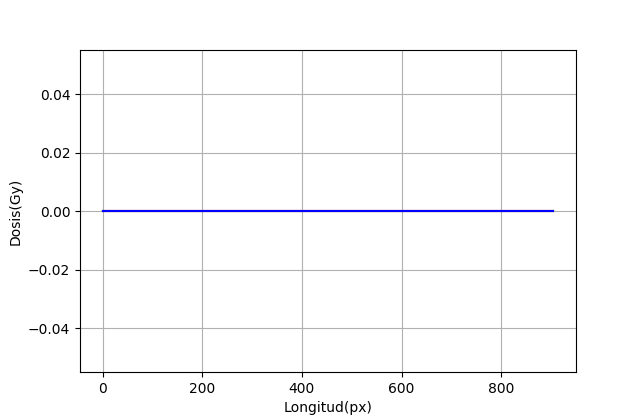
\includegraphics[width=0.7\linewidth]{images/perfilHorizontalDeDosisCeroMulticanal.png}
	\caption{Perfil de dosis horizontal en película sin irradiar con método multicanal }
	\label{fig:perfilCero}
\end{figure}

También, se produjo la separación de las componentes independientes de dosis en la película sin irradiar, las cuales se muestran en la figura \ref{fig:irregularCero}. En esta se evidencian las inhomogeneidades de la película, así como defectos propios del escáner utilizado.\\ 
\begin{figure}[H]
	\centering
	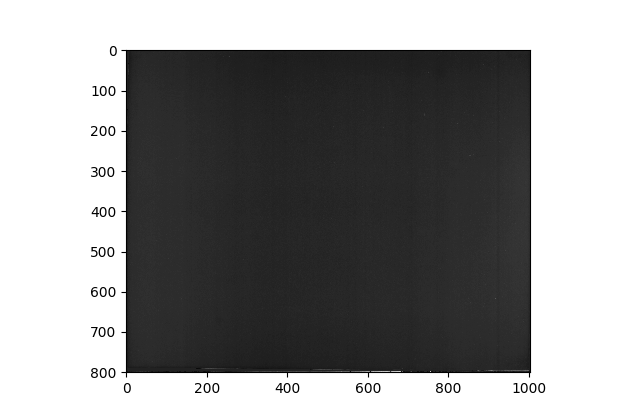
\includegraphics[width=0.7\linewidth]{images/fondoIndependienteDosisPeliculaCero.png}
	\caption{Irregularidades en película sin escanear obtenidas con método multicanal }
	\label{fig:irregularCero}
\end{figure}

Por otro lado, también se investigó la diferencia en ruido al usar canales de color de 8 o 16 bits. En la figura  \ref{fig:8o16} se muestran perfiles centrales para el cuadrado de 5 Gy, cuando la película se escanea en modo de 8 y 16 bits. Aquí, se evidencia que usando 8 bits se presentan mayores diferencias entre las dosis calculadas en cada canal debido a la menor capacidad de diferenciar colores. Se encontró que, contrario a lo que se esperaba, usar 8 bits de profundidad por canal de color presenta más ruido en la determinación de la dosis que usar canales de 16 bits. Esto posiblemente se debe a que la parte más significante del ruido provenga de la fase de digitalización y no de variables físicas como las imperfecciones en el escáner. \\
\begin{figure}[H]
	\centering
	\subfloat[Perfil de dosis central con profundidad de 8 bits]{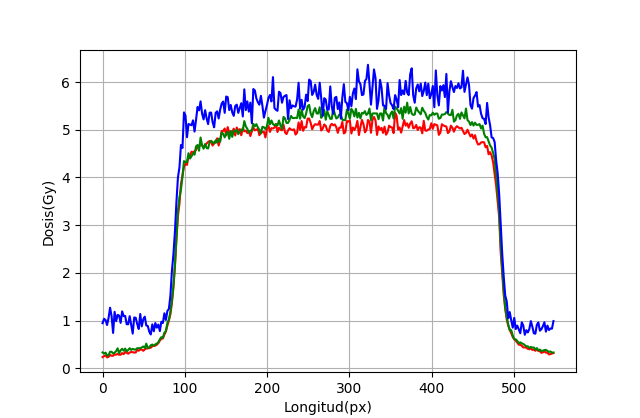
\includegraphics[width=0.7\textwidth]{images/perfilCuadradoMenosBit.png}\label{fig:perfil8}}
	\hfill
	\subfloat[Perfil de dosis central con profundidad de 16 bits ]{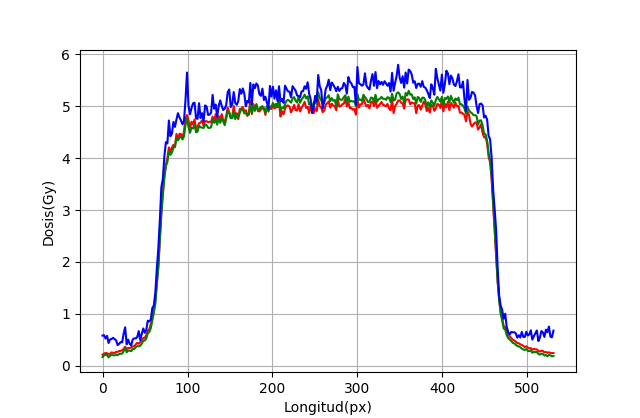
\includegraphics[width=0.7\textwidth]{images/perfilDosisCuadradoUnoSolo.png}\label{fig:perfil16}}
	\caption{Perfil central de dosis en película con cuadrado de 5 Gy a 8 y 16 bits de profundidad de color}
	\label{fig:8o16}
\end{figure}

Finalmente, se comprobó la dependencia de la transmitancia medida en el escáner dependiendo de la orientación de la película con respecto a la lámpara de escaneo, provocada por la polarización que ocurre en la medida. Este efecto se ve en las curvas de calibración presentadas en la figura \ref{fig:efectoOrientacion}, en las cuales se evidencia un desplazamiento en las transmitancias promedio cuando se rota la misma película 90 grados en la misma posición de escaneo.\\
\begin{figure}[H]
	\centering
	\subfloat[Curva de calibración con películas sin rotar]{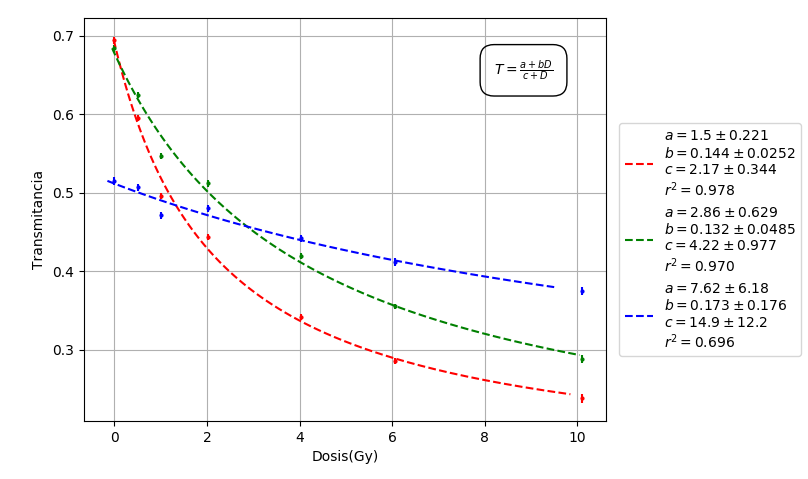
\includegraphics[width=0.7\textwidth]{images/calibracion0-20-sinRotar.png}\label{fig:sinRotar}}
	\hfill
	\subfloat[Curvas de calibración con películas rotadas 90 grados ]{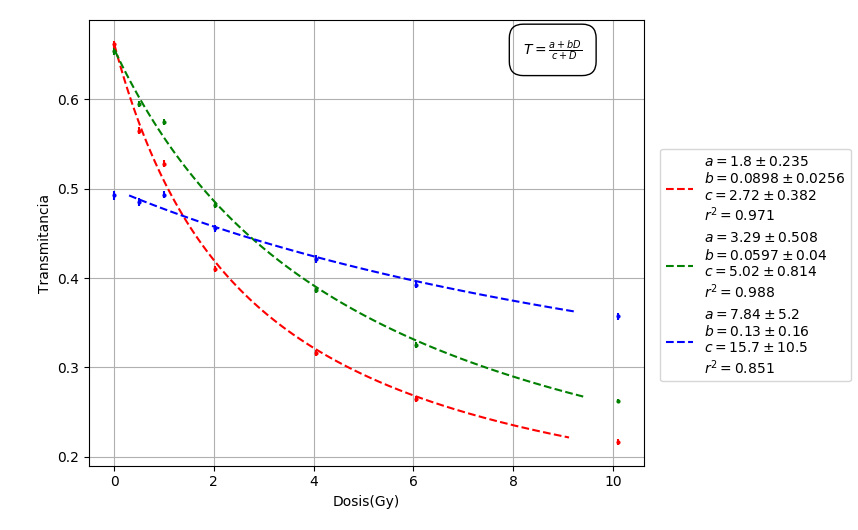
\includegraphics[width=0.7\textwidth]{images/calibracion0-20-Rotadas.png}\label{fig:perfil16}}
	\caption{Efecto de la orientación de escaneo sobre las transmitancias medidas}
	\label{fig:efectoOrientacion}
\end{figure}
Este efecto no es significativo en las medidas tomadas siempre y cuando se procuren orientar las películas cada vez en la misma dirección con respecto a la lámpara del escáner.\\

No fue posible comprobar el efecto de otras variables como la temperatura y el tiempo post-exposición, dadas las restricciones de tiempo y movilidad que se presentaron en el transcurso del trabajo, además de la poca capacidad de control que se tiene sobre estas variables en el transcurso del proceso.\\

\section{Mapas de dosis}


El plan piramidal de prueba produjo una película resultante que se ilustra en la figura \ref{fig:piramideEscaneada}.\\
\begin{figure}[H]
	\centering
	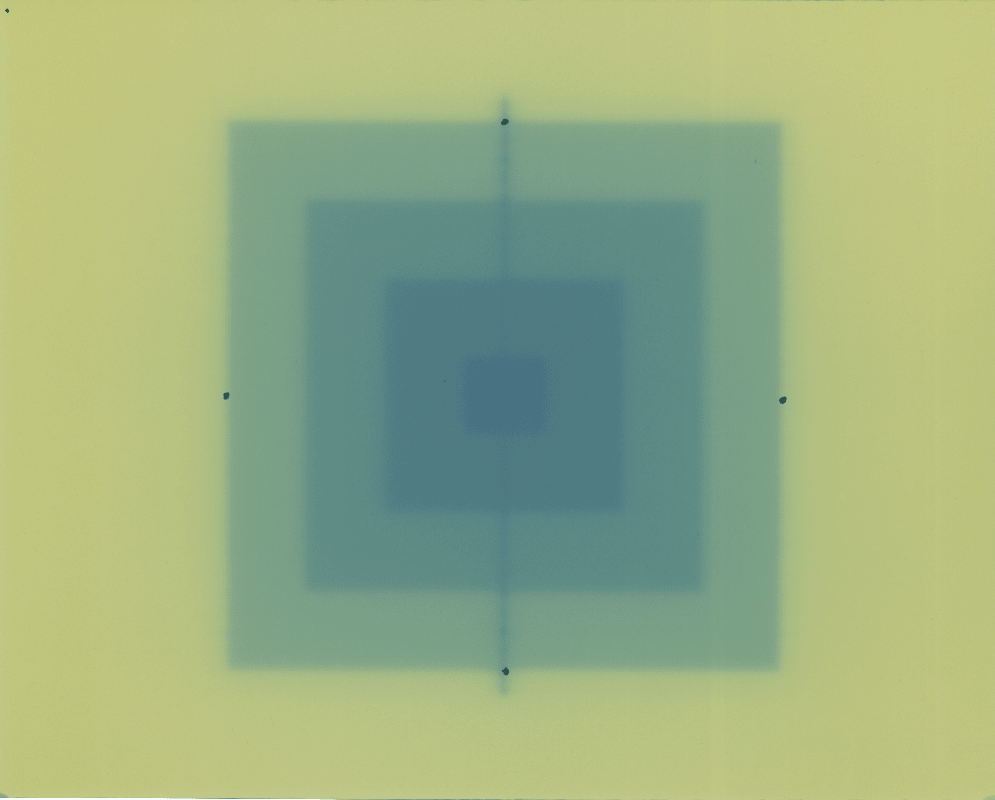
\includegraphics[width=0.7\linewidth]{images/peliculaPiramide.png}
	\caption{Película EBT3 irradiada con plan de pirámide }
	\label{fig:piramideEscaneada}
\end{figure}

En la figura \ref{fig:mapaPiramide} se muestra el mapa de dosis calculado con la digitalización anterior, junto con la parte independiente de dosis que proporciona el método multicanal.\\

\begin{figure}[H]
	\centering
	\subfloat[Mapa de dosis obtenido para el plan pirámide]{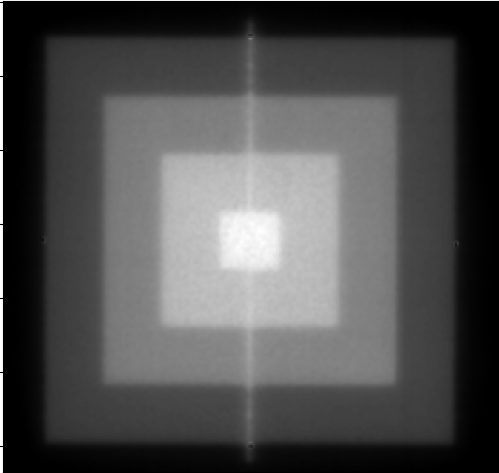
\includegraphics[width=0.5\textwidth]{images/mapaDosisPiramidePelicula.png}\label{fig:mapaPiramideFInal}}
	\hfill
	\subfloat[Parte independiente de dosis para el plan pirámide ]{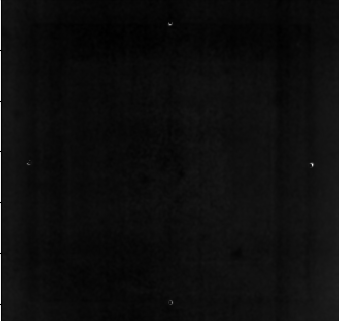
\includegraphics[width=0.5\textwidth]{images/fondoIndependienteMapaPiramide.png}\label{fig:indepPiramide}}
	\caption{Mapa de dosis escaneado para el plan pirámide}
	\label{fig:mapaPiramide}
\end{figure}

Se pueden usar diversas herramientas para comparar estos planes, por ejemplo, en la figura \ref{fig:perfilesDosisPiramide} se muestran perfiles de dosis a diferentes niveles que muestran una concordancia entre las dosis calculadas en ambos mapas. Esta concordancia es aproximada, presentando una ligera subestimación de la dosis planeada usando la película escaneada. Esto podría deberse a factores como el ruido en la imagen y las condiciones de escaneo. Sin embargo, es evidente la concordancia espacial que se presenta en ambas.\\
\begin{figure}[H]
	\centering
	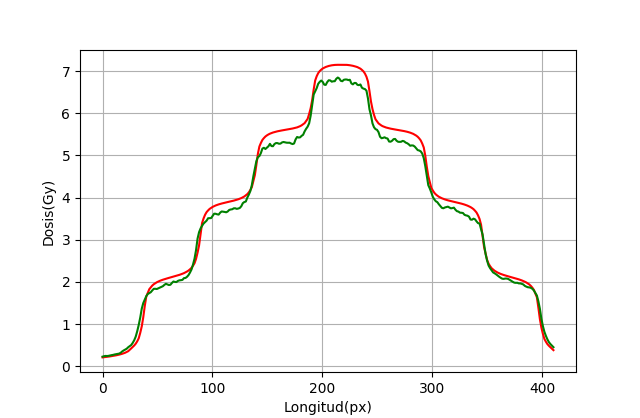
\includegraphics[width=0.7\linewidth]{images/perfilCentralPiramide.png}
	
	\caption{Perfiles central de dosis para plan pirámide }
	\label{fig:perfilesDosisPiramide}
\end{figure}
Es útil comparar estos mapas normalizados con respecto a un valor. De esta manera, aunque se pierda información relativa a la dosis depositada en cada punto, es más efectiva para comprobar similitudes en las distribuciones espaciales de las dosis entregadas. Un perfil de dosis normalizado se muestra en la figura \ref{fig:perfilesDosisPiramideNorm}, en este caso se normaliza con respecto al máximo de dosis en cada mapa.\\
\begin{figure}[H]
	\centering
	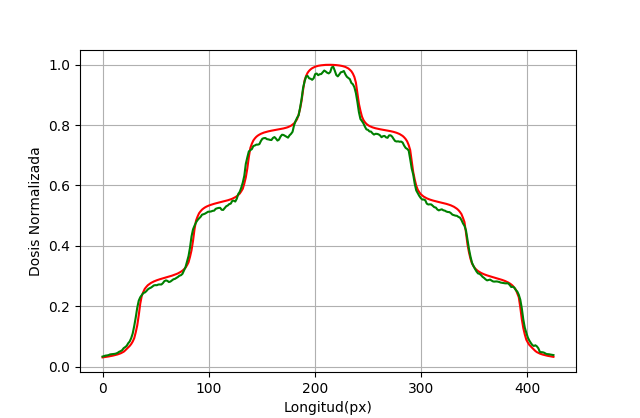
\includegraphics[width=0.7\linewidth]{images/perfilPiramideNormalizado.png}
	
	\caption{Perfiles central de dosis normalizado para plan pirámide. }
	\label{fig:perfilesDosisPiramideNorm}
\end{figure}

Con este perfil se evidencia que el mapa producido con la película corresponde de buena manera con el mapa calculado con por el TPS.\\

Por otro lado, en la figura \ref{fig:isodosisPiramide}  se presentan curvas de isodosis de estos mapas para tres porcentajes sobre el valor de normalización. Estos porcentajes se muestran en la parte inferior de la figura y son ajustables manualmente en la pantalla del computador. En línea sólida se muestran las isodosis calculadas sobre el mapa producido por el TPS, mientras que en lineas punteadas se muestran las isodosis con el mismo porcentaje de dosis, pero calculadas con respecto al mapa obtenido con la película. En este caso, cada mapa está normalizado con respecto a la dosis máxima en cada uno. \\ 
\begin{figure}[H]
	\centering
	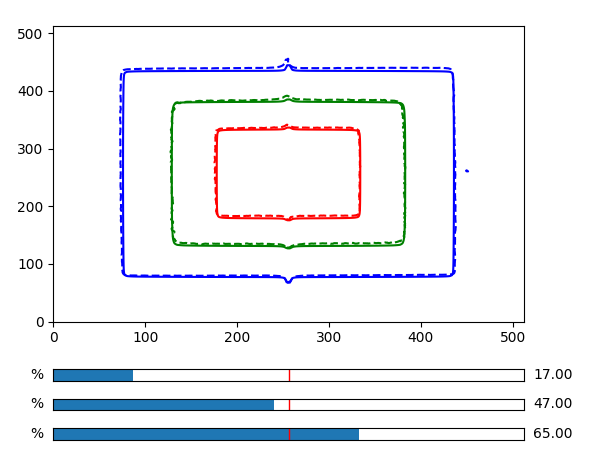
\includegraphics[width=0.7\linewidth]{images/isodosisPiramide2.png}
	\caption{Curvas de isodosis para el plan pirámide calculadas sobre el TPS y la película escaneada.  }
	\label{fig:isodosisPiramide}
\end{figure}

Se evidencia que las formas de las isodosis concuerdan, aunque también se hace presente la gran cantidad de ruido en los mapas producidos con las películas, aún cuando se aplicaron filtros sobre estas para reducirlo. Esta cantidad de ruido es inesperado y podría deberse a a la calidad del escáner usado. \\

Así mismo, se realiza un análisis comparativo del plan de tratamiento de mama, que produjo la película que se muestra en la figura \ref{fig:mamaEscaneada}.\\
\begin{figure}[H]
	\centering
	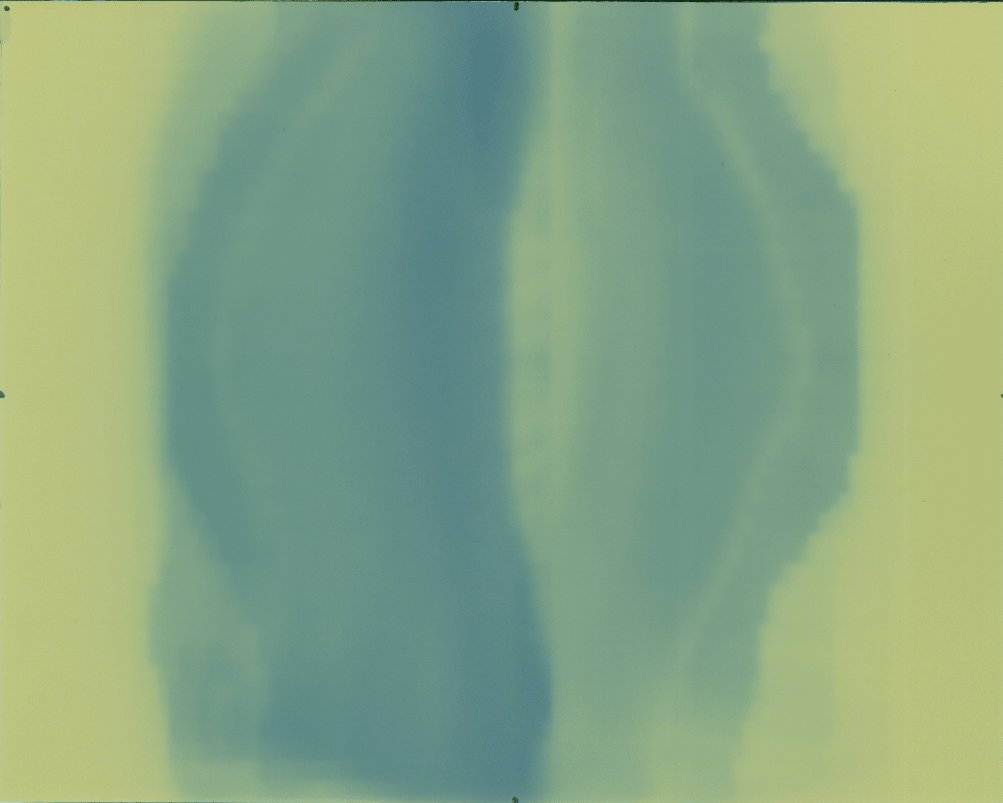
\includegraphics[width=0.7\linewidth]{images/peliculaMama.png}
	\caption{Película EBT3 irradiada con plan de tratamiento de mama. }
	\label{fig:mamaEscaneada}
\end{figure}
Usando el método multicanal, se obtiene el mapa de dosis que se muestra en la figura \ref{fig:mapaMAma} , junto con la parte independiente de dosis de la película.
\begin{figure}[H]
	\centering
	\subfloat[Mapa de dosis obtenido para el plan de mama.]{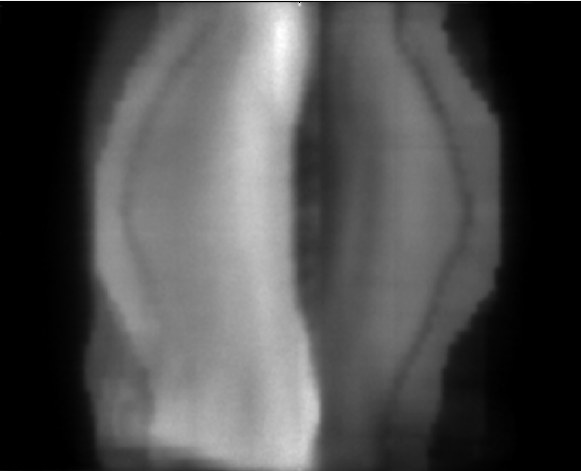
\includegraphics[width=0.5\textwidth]{images/mapaDosisMamaPelicula.png}\label{fig:mapaMAmaFInal}}
	\hfill
	\subfloat[Parte independiente de dosis para el plan de tratamiento de mama. ]{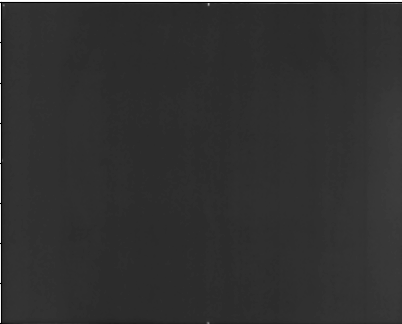
\includegraphics[width=0.5\textwidth]{images/fondoIndependienteMama.png}\label{fig:indepMama}}
	\caption{Mapa de dosis escaneado para el plan de tratamiento de mama.}
	\label{fig:mapaMAma}
\end{figure}

En la figura \ref{fig:mamaPerfil} se muestra un perfil de dosis normalizado horizontal que pasa por la parte central del plan para los mapas calculado por el TPS y obtenido con la película. Se evidencia la concordancia relativa entre ambos perfiles, aunque por la complejidad del plan, que involucra un movimiento continuo de las láminas del MLC, en comparación del plan pirámide, donde estas permanecen estáticas, se observa mayor dispersión con respecto al perfil obtenido en el plan pirámide.\\

\begin{figure}[H]
	\centering
	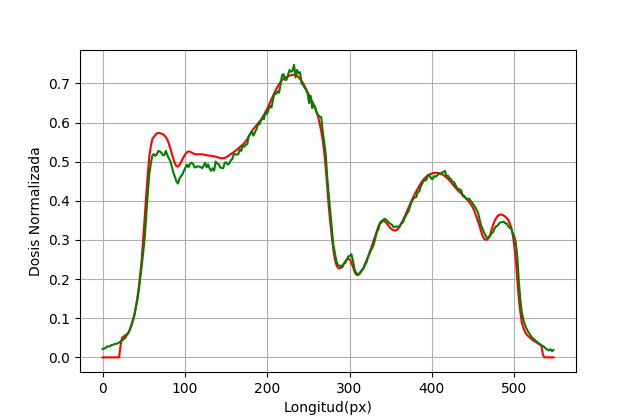
\includegraphics[width=0.7\linewidth]{images/perfilDosisMama.png}
	\caption{Perfil en el plan de tratamiento de mama. }
	\label{fig:mamaPerfil}
\end{figure}

Del mismo modo, en la figura \ref{fig:mamaIsodosis} se muestran tres curvas de isodosis comparadas con las producidas por el TPS y las obtenidas con la película. También se evidencia una concordancia entre estas, aunque un poco más distorsionadas por el ruido en la película.

\begin{figure}[H]
	\centering
	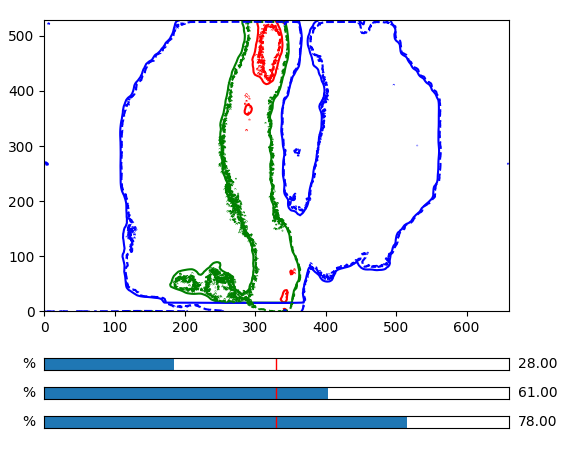
\includegraphics[width=0.7\linewidth]{images/curvasIsodosisMama.png}
	\caption{Curvas de isodosis superpuestas para el plan de tratamiento de mama }
	\label{fig:mamaIsodosis}
\end{figure}

\section{Comparaciones $\Gamma$}

Para comprobar la implementación del cálculo de $\Gamma$, se compararon los planes que se muestran en la figura \ref{fig:barraAtravesa} con un análisis gamma de 1 mm y 1\%. Esto se realizó mediante el programa IBA, del fabricante IBA Dosimetry \footnote{https://www.iba-dosimetry.com}, y el implementado en el desarrollo propio con la liberia phymedphys de python.

\begin{figure}[H]
	\centering
	\subfloat[Mapa piramidal con una lámina del MLC puesta]{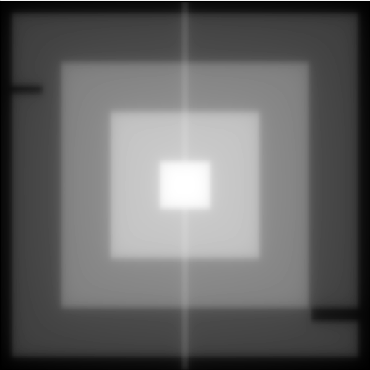
\includegraphics[width=0.5\textwidth]{images/piramideAtravesada}\label{fig:mapaPiramideAtrav}}
	\hfill
	\subfloat[Mapa piramidal sin la lámina del MLC ]{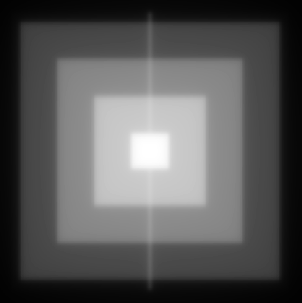
\includegraphics[width=0.5\textwidth]{images/piramideTPS2.png}\label{fig:mapaPiramideA}}
	\caption{Planes para testeo de implementación del cálculo $\Gamma$}
	\label{fig:barraAtravesa}
\end{figure}

Las matrices gamma obtenidas con ambas implementaciones concuerdan y se muestran en la figura \ref{fig:barraAtravesaGamma}. El porcentaje de aprobación de pixeles es del 97\% calculado por ambos programas, lo que permite asegurar que la implementación es correcta. Además, se resalta que la matriz gamma identifica plenamente las regiones donde se presentan las diferencias importantes entre planes. 

\begin{figure}[H]
	\centering
	\subfloat[Matriz $\Gamma$ obtenida con el programa IBA]{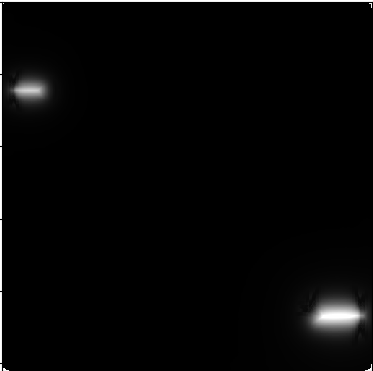
\includegraphics[width=0.5\textwidth]{images/gammaAtravesada.png}\label{fig:GammaIBA}}
	\hfill
	\subfloat[Matriz $\Gamma$ obtenida con la implentación phymedphys ]{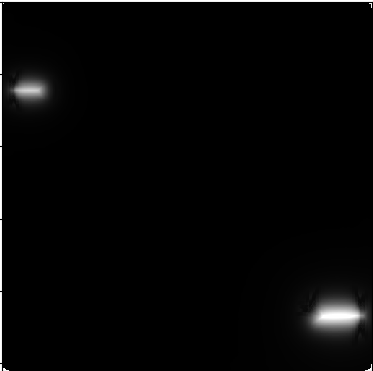
\includegraphics[width=0.5\textwidth]{images/gammaAtravesada.png}\label{fig:GammaPropio}}
	\caption{Matrices $\Gamma$ calculadas con dos implementaciones}
	\label{fig:barraAtravesaGamma}
\end{figure}

Una vez comprobada la efectividad en el cálculo de $\Gamma$, se procede a realizar el mismo análisis sobre los planes escaneados. En el caso del plan pirámide, se obtiene la matriz $\Gamma$ mostrada en la figura \ref{fig:matrixGAmmaPiramide}, y en la figura \ref{fig:histogramaGAmmaPiramide} se muestra el histograma de $\Gamma$ que evalúa la correspondencia general de los pixeles en ambas distribuciones.\\

\begin{figure}[H]
	\centering
	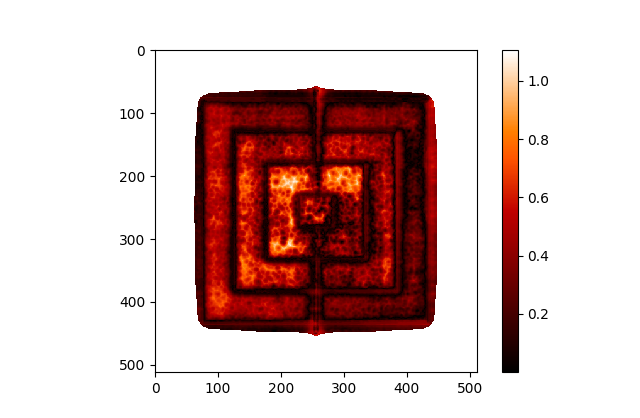
\includegraphics[width=0.9\linewidth]{images/gammaPiramideCalor.png}
	\caption{Matriz $\Gamma$ obtenida para el plan de tratamiento piramidal }
	\label{fig:matrixGAmmaPiramide}
\end{figure}
\begin{figure}[H]
	\centering
	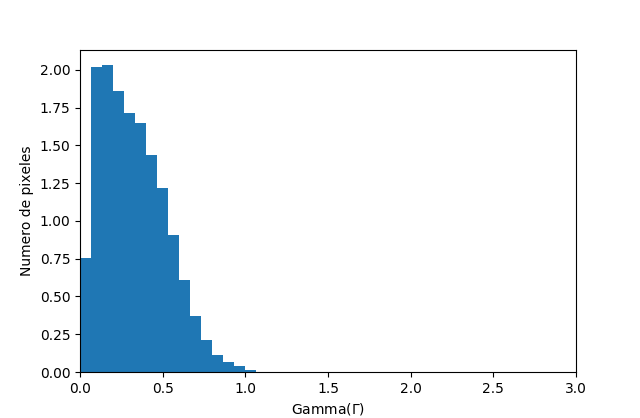
\includegraphics[width=0.9\linewidth]{images/histogramaGammaPiramide.png}
	\caption{Histograma $\Gamma$ obtenida para el plan de tratamiento piramidal  }
	\label{fig:histogramaGAmmaPiramide}
\end{figure}

Se evidencia una correspondencia del 97\% bajo un análisis de $\Gamma$ de 2mm y 2\%, omitiendo los pixeles cuyo valor es menor a 5\% del máximo en cada plan. Esto permite concluir que el plan ejecutado corresponde en gran medida con el planeado en el TPS, aún teniendo en cuenta la gran cantidad de ruido  que tiene el mapa producido con la película. Esto es de esperar, dada la simplicidad de este plan de prueba, en la que la simulación que realiza el sistema de planeación corresponde muy bien con las condiciones reales en las que se ejecuta la irradiación.\\

Finalmente, en el caso del plan de tratamiento de mama, se muestra el mismo análisis $\Gamma$ bajo los mismos parámetros. En la figura \ref{fig:matrixGAmmaMAma} se encuentra la matriz $\Gamma$ calculada para este plan con respecto a la película escaneada. Y en la figura \ref{fig:histogramaGAmmaMama} se muestra el histograma de los valores de gamma en los pixeles. En este caso, el porcentaje de aprobación es de 87\%, menor que el obtenido en el plan pirámide. Esto es de esperar por la mayor complejidad del plan, el ruido en la película, y la dificultad para superponer manualmete los mapas de dosis, lo que induce una desviación muy grande en el resultado final.\\

\begin{figure}[H]
	\centering
	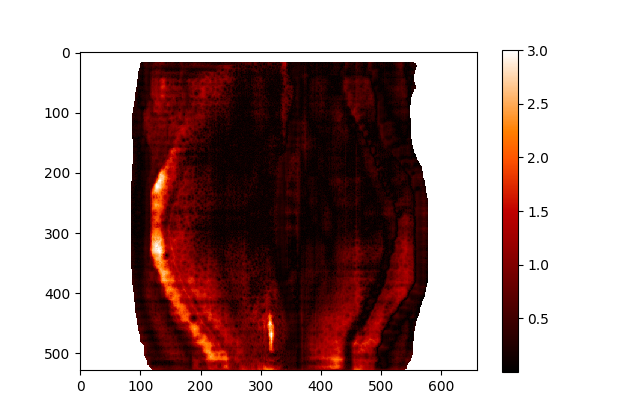
\includegraphics[width=0.7\linewidth]{images/gammaMama.png}
	\caption{Matriz $\Gamma$ obtenida para el plan de tratamiento de mama }
	\label{fig:matrixGAmmaMAma}
\end{figure}
\begin{figure}[H]
	\centering
	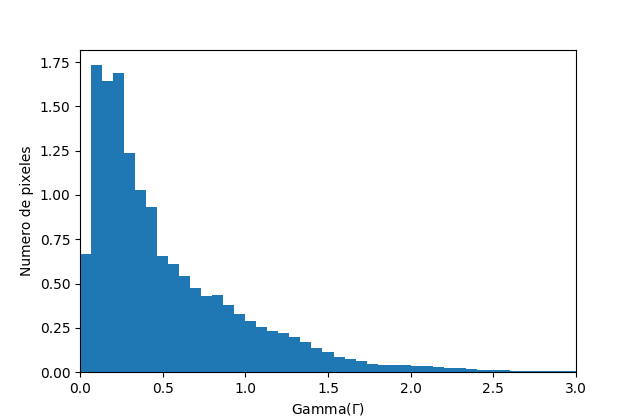
\includegraphics[width=0.7\linewidth]{images/histogramaDosisMama.png}
	\caption{Histograma $\Gamma$ obtenida para el plan de tratamiento de mama  }
	\label{fig:histogramaGAmmaMama}
\end{figure}

Estaba planeado realizar comparaciones para estos planes con mapas de fluencias producidos con dosimetría portal con detectores de silicio, sin embargo, esto no fue posible dadas las restricciones de tiempo, además de la incapacidad de traducir los mapa de fluencias obtenidos con este tipo de dispositivos en mapa de dosis.\\

En el apéndice A se muestran diagramas de flujo que resumen el funcionamiento del programa. En el apéndice B se esquematizan las diferentes ventanas que se implementaron en la interfaz para el programa.\\ 





